\documentclass{article}
\usepackage{graphicx} % Required for inserting images

\documentclass[a4paper, 12pt]{article}%тип документа

%отступы
\usepackage[left=2cm,right=2cm,top=2cm,bottom=3cm,bindingoffset=0cm]{geometry}
\usepackage[pdftex]{lscape}
%Русский язык
\usepackage[T2A]{fontenc} %кодировка
\usepackage[utf8]{inputenc} %кодировка исходного кода
\usepackage[english,russian]{babel} %локализация и переносы
\usepackage{multirow}
%Вставка картинок
\usepackage{wrapfig}
\usepackage{graphicx}
\graphicspath{{Images/}}
\DeclareGraphicsExtensions{.pdf,.png,.jpg}

%Математика
\usepackage{amsmath, amsfonts, amssymb, amsthm, mathtools}

%Заголовокhttps://www.overleaf.com/project/6507f5a4176b25bf05722230

\begin{document}

\begin{titlepage}
	\begin{center}
		{\large МОСКОВСКИЙ ФИЗИКО-ТЕХНИЧЕСКИЙ ИНСТИТУТ (НАЦИОНАЛЬНЫЙ ИССЛЕДОВАТЕЛЬСКИЙ УНИВЕРСИТЕТ)}
	\end{center}
	\begin{center}
		{\large Физтех-школа биологической и медицинской физики}
	\end{center}
	
	
	\vspace{4.5cm}
	{\huge
		\begin{center}
			{\bf Отчёт о выполнении лабораторной работы}\\
			Газо-адсорбционная хроматография
		\end{center}
	}
	\vspace{3cm}
	\begin{flushright}
		{\LARGE Авторы:\\ Акимов Максим \\ Кондратюк Наталья \\
			\vspace{0.5cm}
			Б06-206}
	\end{flushright}
	\vspace{3cm}
	\begin{center}
		Долгопрудный 
       \\14 октября 2024 года
	\end{center}
 
\end{titlepage}

\newpage 
\section{Аннотация}

\paragraph*{Цель работы}: Изучить метод газо-адсорбционной хроматографии и применить его к расчётам термодинамических характеристик исследуемых веществ, а также для проверки модели теоретической тарелки.

\paragraph*{Задачи}:
\begin{itemize}
    \item ознакомиться с содержанием работы; разобраться с работой хроматографа и необходимым ПО;
    \item определить теплоту адсорбции изучаемых веществ (смеси воды, этилового и метилового спиртов) по полученным данным; отметить влияние $-CH_2$ группы на данную величину;
    \item провести расчёт разрешающей способности хроматографа; провести необходимые расчёты и построения согласно теории теоретической тарелки;
    \item обработать данные, сделать выводы о соответствии результатов теоретически ожидаемым, сделать выводы о работе в целом, сдать и оформить отчёт о выполнении лабораторной работы.
\end{itemize}
\section{Введение}
\subsection{Изотерма сорбции}\;
\par Метод газо-адсорбционной хроматографии основан на явлении адсорбции молекул из газовой фазы на поверхности твёрдого тела, то есть повышении концентрации на границе раздела фаз.
\begin{wrapfigure}{l}{0.3\textwidth}
    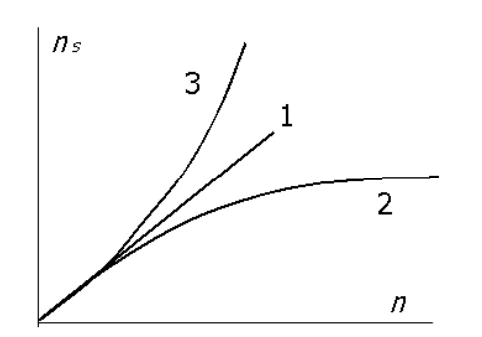
\includegraphics[width=0.3\textwidth]{Images/адсорбция.png}
    \caption{Наблюдаемые изотермы сорбции: 1 - изотерма Генри,
2 - изотерма Ленгмюра, 3 - изотерма полислойной адсорбции.}
\end{wrapfigure} \;
\par Уравнение, связывающее (при постоянной температуре) поверхностную концентрацию адсорбированных молекул $n_{S}$ с их объемной концентрацией n в подвижной фазе (ПФ), называется изотермой сорбции. Изотерма Генри выводится из предположения об установлении адсорбционно-десорбционного равновесия:
\begin{equation}
\frac{n_S}{n} = \frac{k_a}{k_d} = \frac{v_T}{4}*\tau_0 * \exp \frac{Q}{T} \Rightarrow n_S = \chi n,
\label{exp_Q}
\end{equation}
где $\chi$ - константа Генри, $\tau_0 = 1/k_0$ - характерное время колебания адсорбированной молекулы, $v_T$ - средняя скорость теплового движения молекул, а $Q$ - теплота адсорбции.
\par Модель Ленгмюра учитывает конечность числа связывающих центров на твердой поверхности. Вводится понятие степени заполнения поверхности $\theta$ как отношения заполненных мест связывания $n_S$ к полному числу центров адсорбции $n_{lim}$. Изотерма Ленгмюра выводится из условия равенства скоростей сорбции и десорбции:
\begin{equation}
\theta = \frac{k_a n}{k_a n + k_d n_{\lim}} = \frac{1}{1 + \frac{B}{n}},
\end{equation}
где $B = \frac{k_d}{k_a}*n_{\lim}$ - комбинация констант.

\par Адсорбционно-десорбционные процессы на поверхности твердого тела существенно зависят от величины энергии Q, называемой теплотой адсорбции. Теплота адсорбции определяется вкладом различных типов взаимодействий, которые реализуются между молекулами адсорбата и адсорбента. Величина Q при хемосорбции достигает 100 кДж/моль, а для физической адсорбции не превышает нескольких десятков кДж/моль.
\subsection{Время удерживания и высота эквивалентной теоретической тарелки}\;
\par Время пребывания молекулы в хроматографической колонке $t_1$ (называемое временем удерживания) складывается из времени движения $t_0$ в ПФ и времени неподвижного пребывания $t_S$ в неподвижной фазе (НФ). Из равенства средних скоростей сорбции и десорбции можно получить, что:
\begin{equation}
t_1 = t_0 ( 1 + \frac{2n_S}{\rho n}),
\end{equation} 
где $\mu = \frac{t_S}{t_0} = \frac{2}{\rho} \chi$
\par Эффективное разделение веществ методом хроматографии достигается при условии достаточно сильной адсорбции, поэтому обычно $\mu \gg 1$ и тогда $t_1 \sim t_0 \mu$. Обозначая линейную скорость газа-носителя $v_0$, для времени пребывания молекул в ПФ получаем:
\begin{equation}
t_0 = \frac{L}{v_0}.
\end{equation}

\begin{figure}[h!]
    \centering
    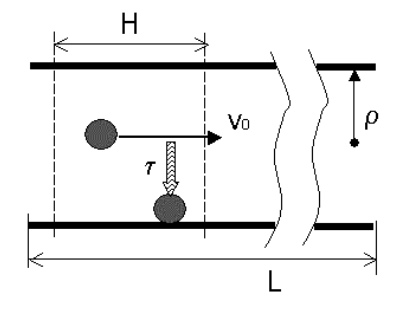
\includegraphics[width=0.5\linewidth]{Images/ВЭТТ.png}
    \caption{Иллюстрация понятия высоты эквивалентной теоретической тарелки (ВЭТТ)}
    \label{fig:ВЭТТ}
\end{figure}
\par Высота, эквивалентная теоретической тарелке (ВЭТТ) равна длине участка хроматографической колонки, на котором успевает установиться адсорбционно-десорбционное равновесие между молекулами в ПФ и НФ (Рис. \ref{fig:ВЭТТ}). Полагая, что время установления равновесия $\tau$
определяется временем диффузии молекул из объема к поверхности, получим оценку:
\begin{equation}
\tau \sim \frac{\rho^2}{D}.
\end{equation}
Если ввести обозначение Н для ВЭТТ, то:
\begin{equation}
H = v_0 \tau, 
\end{equation} 
а количество теоретических тарелок r в колонке длиной L, составит
\begin{equation}
r = \frac{L}{H}.
\end{equation}

\subsection{Уравнение Ван-Деемтера}\;
\par Уравнение Ван-Деемтра позволяет рассмотреть зависимость ВЭТТ от скорости потока газаносителя, что очень удобно на практике, так как регулировка потока производится очень просто. Так как ВЭТТ пропорциональна числу теоретических тарелок: $H \sim 1/r$, $R^2 \sim r$, следовательно, $H \sim 1/R^2$. Тогда получим:
\begin{equation}
H \sim ( \sqrt{\frac{v_0 \rho^2}{LD}} + \sqrt{\frac{2S}{Lv_0}} ) ^2 =  Av_0 + \frac{B}{v_0} + C.
\end{equation}
\par Минимум этой функции означает, что существует оптимальная скорость потока при которой достигается максимальная разрешающая способность хроматографической колонки.
\section{Описание установки}\;
\par Работа производилась на хроматографе "ЦВЕТ - 800", на его примере и рассмотрим устройство прибора (Рис. \ref{fig:схема}). Разделение веществ происходит в стальной насадочной колонке длиной 2 м и диаметром 3 мм, заполненной порапаком. В неё подаётся газ-носитель (в нашем случае гелий), который служит подвижной фазой.
\par Гелий из балона поступает через редуктор в блок подготовки газов, который поддерживает стабильный объёмный расход в мл/мин. Затем с помощью дозирующего крана (Рис. \ref{fig:кран}) проба вводится в поток. В режиме "ОТБОР" петля крана продувается анализируемым веществом, а в положении "АНАЛИЗ" заполненная петля вводится в поток газа-носителя. Перед попаданием в колонку проба проходит через испаритель для полного перевода в газовую фазу, а только затем разделяется. На выходе из колонки стоит детектор, работающий на разности теплопроводностей чистого газа-носителя и анализируемого вещества. Управление режимом работы прибора и обработка пиков на хроматограмме производится в программе "Цвет-Аналитик".
\begin{figure}[!htb]
                \minipage{0.6\textwidth}
                 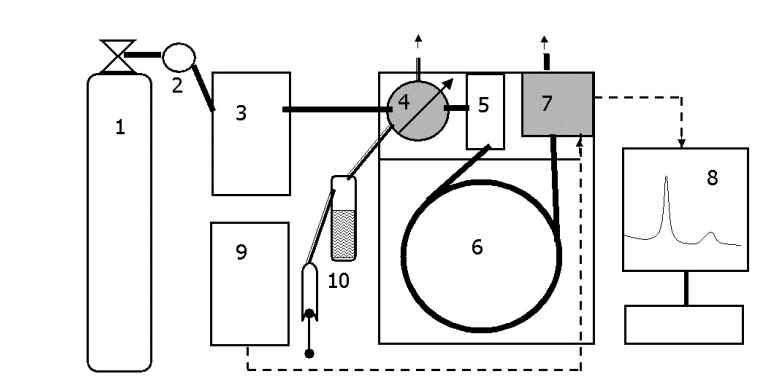
\includegraphics[width=\linewidth]{Images/схема хроматографа.png}
                 \label{fig:схема}
                 \caption{Блок-схема хроматографа}
                  \endminipage\hfill
                \minipage{0.4\textwidth}
                 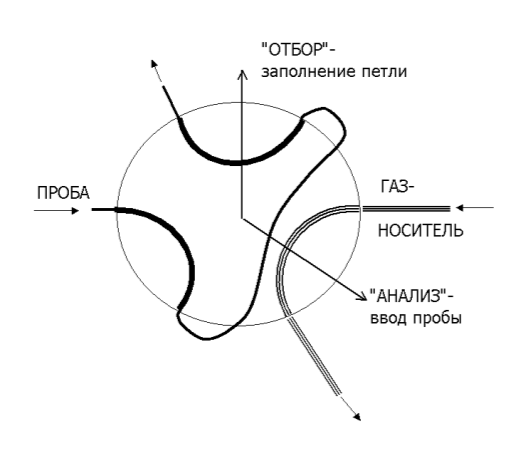
\includegraphics[width=\linewidth]{Images/кран-дозатор.png}
                 \label{fig:кран}
                 \caption{Устройство крана-дозатора}
                  \endminipage
\end{figure}
\section{Результаты и обсуждение}
\subsection{Определение теплоты адсорбции воды и спиртов на сорбенте}\;

    \par Проведя серии экспериментов, получим хроматограммы проб со смесью спиртов при нескольких значениях температуры колонки в диапазоне $130 - 180 ^{\circ}C$ и постоянной скорости газа носителя $30$ мл/мин.
    
     Определим времена удерживания $t_1$ для воды, метанола и этанола при различной температуре (Таблица \ref{Разные температуры}). В качестве $t_0$ принять время удерживания $N_2$ и $O_2$, которые можно считать несорбирующимися компонентами.

    \begin{table}[h!]
    \centering
    \caption{Данные хроматограмм при разных температурах}
    \begin{tabular}{|l|l|l|l|l|l|l|l|l|}
    \hline
    $T,\; K$ & $\frac{1}{T}\cdot 10^3,\; \frac{1}{K} $ & $t_1(H_2O),\;$ с & $\ln{(H_2O)}$ & $t_1(CH_3OH),\;$ с & $\ln{(CH_3OH)}$ & $t_1(C_2H_5OH),\;$ с & $\ln{(C_2H_5OH)}$ & $t_0,\;$ с \\ \hline
 403&  2,48& 208,60 
& -0,80
&  290,72&  -0,43&  622,28&  0,37&  20,76 
\\ \hline
 413&  2,42& 164,12 
& 
-1,07
&  218,44&  -0,74&  442,68&  0,01&  20,56 
\\ \hline
 423&  2,36& 131,60 
& -1,28
&  168,16&  -0,99&  320,80&  -0,29&  19,60 
\\ \hline
 433&  2,30& 107,04 
& 
-1,50
&  133,36&  -1,24&  240,88&  -0,58&  19,00 
\\ \hline
 443&  2,25& 90,16 
& -1,70
&  108,12&  -1,48&  185,64&  -0,85&  18,64 
\\ \hline
 453&  2,20& 77,36 & 
-1,92
&  90,40&  -1,72&  146,05&  -1,14&  18,72 \\ \hline
\end{tabular}
\label{Разные температуры}
\end{table}
    Используя теоретические соотношения, выведем уравнения для нахождения теплот адсорбции:
    
    \begin{equation*}
        \chi = \frac{n_s}{n} = \frac{\upsilon_T}{4}\tau_0 \exp{\frac{Q}{kT}}
    \end{equation*}
    где $\chi$ - константа Генри, $n_s$ - поверхностная концентрация молекул в неподвижной фазе, $n$ - объемная концентрация молекул в подвижной фазе, $\upsilon_T$ - средняя тепловая скорость молекул, $\tau_0$ - характерное время колебания адсорбированной молекулы, $Q$ - теплота адсорбции исследуемого вещества.


    \begin{equation*}
        t_1 = t_0\left(1+\frac{2}{\rho}\frac{n_s}{n}\right)
    \end{equation*} где $t_1$ — время удержания, $\rho$ - радиус колонки, $t_0$ - мертвое время колонки. 

    С учетом $v_T\sim \sqrt{\frac{kT}{m}}$ получаем 
    \begin{equation*}
        \frac{t_1-t_0}{t_0} = \text{const}\cdot \sqrt{T}\exp{\frac{Q}{kT}} \Rightarrow \ln{\left(\frac{t_1-t_0}{t_0} \frac{1}{\sqrt{T}}\right)} = \frac{Q}{k}\frac{1}{T}+const
    \end{equation*}


    Согласно этой зависимости построим график $\ln{\left(\frac{t_1 - t_0}{t_0}\frac{1}{\sqrt{T}}\right)} \left(\frac{1}{T}\right)$ который приведён на Рис. \ref{fig:Рис 1}.

    \begin{figure}[h!]
    \centering
    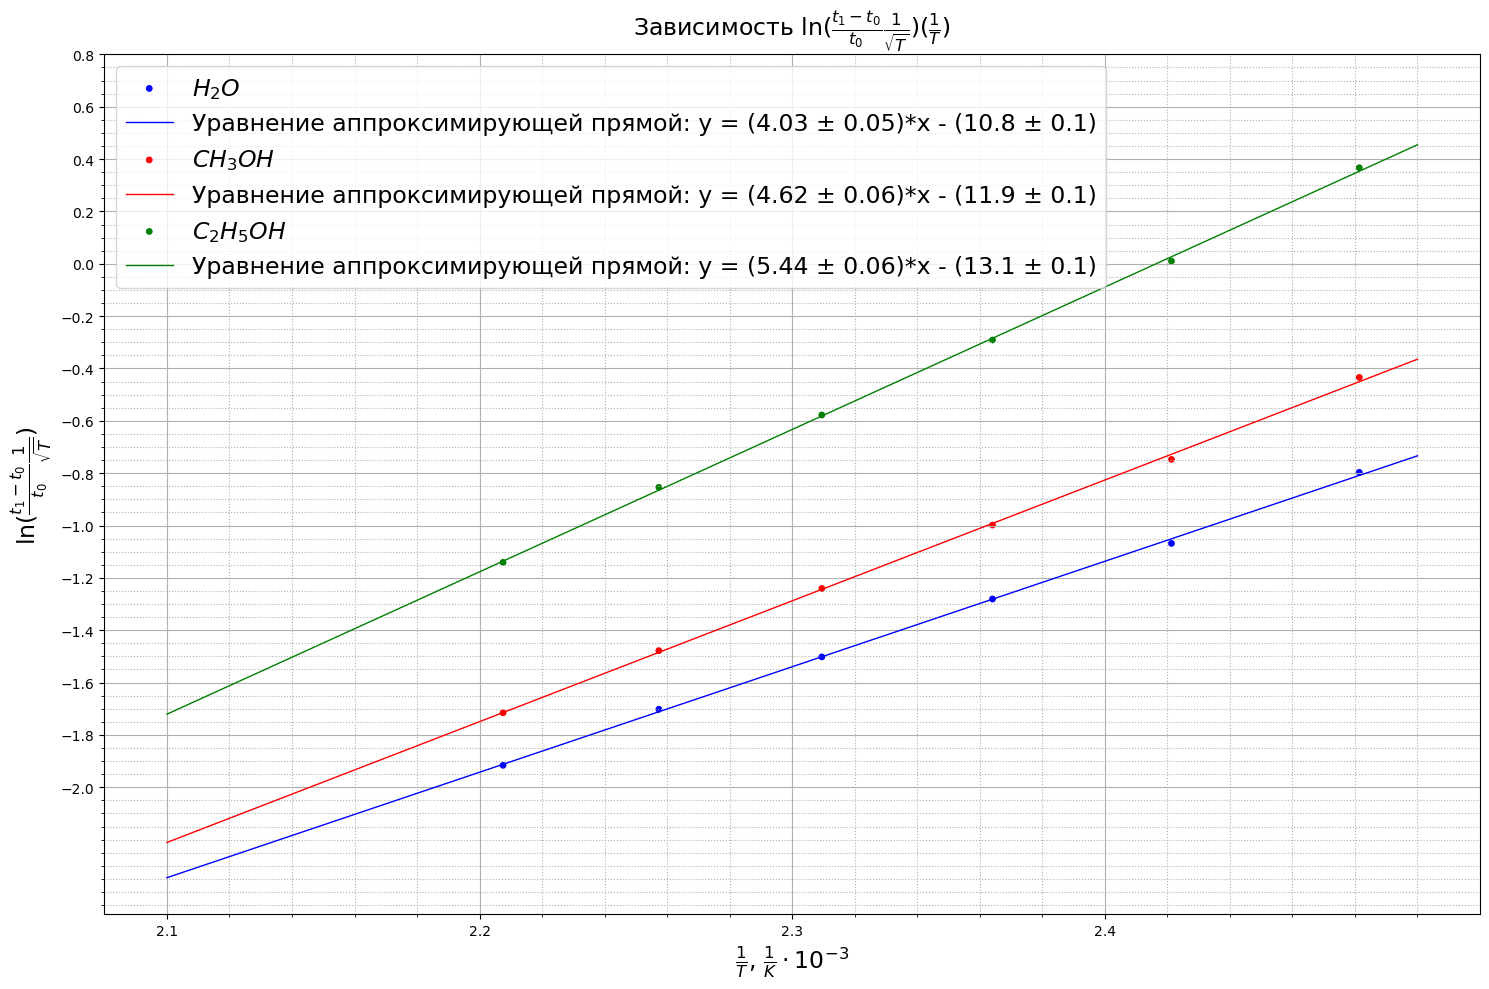
\includegraphics[width=0.75\linewidth]{Images/Зависимость от температуры.png}
    \caption{Зависимость $\ln{\left(\frac{t_1 - t_0}{t_0}\frac{1}{\sqrt{T}}\right)} \left(\frac{1}{T}\right)$ }
    \label{fig:Рис 1}
    \end{figure}

    По полученным коэффициентам наклона определим теплоты адсорбции соответствующих веществ (Таблица \ref{Теплоты адсорбции}).

    \begin{table}[h!]
    \centering
    \caption{Теплоты адсорбции анализируемых веществ}
\begin{tabular}{|l|l|l|l|}
\hline
Вещество & $H_2O$ & $CH_3OH$ & $C_2H_5OH$ \\ \hline
$Q,\;$ кДж/моль & $33,5 \pm 0,4$ & $38,4 \pm 0,5$ & $45,2 \pm 0,5$ \\ \hline
\end{tabular}
\label{Теплоты адсорбции}
\end{table}


Проанализируем полученные данные. Из теплот адсорбции видно, что они растут вместе с увеличением углеродного скелета. Данный ряд теплот, таким образом, отражает влияние группы $-CH_2$ на адсорбцию молекулы на гидрофобном адсорбенте. Следовательно, для самой гидрофильной молекулы воды теплота адсорбции наименьшая. Далее она растёт с увеличением гидрофобной части.





    \begin{figure}[h!]
    \centering
    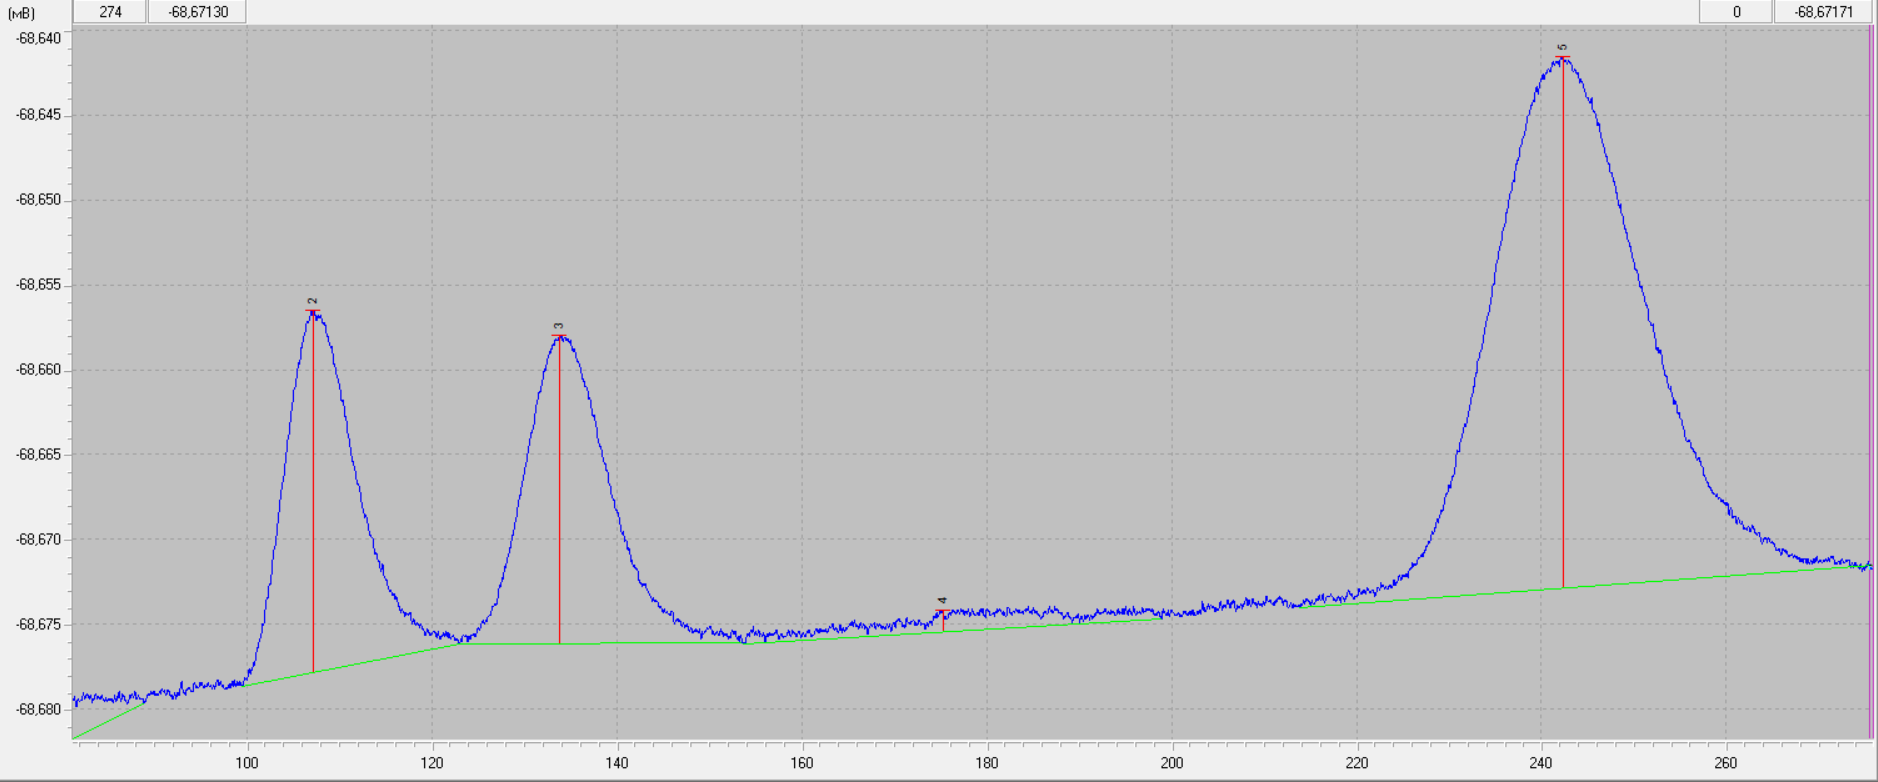
\includegraphics[width=0.75\linewidth]{Images/Снимок экрана 2024-10-13 235735.png}
    \caption{Хроматограмма при 160 $^{\circ}C$ }
    \label{fig:Рис 2}
    \end{figure}

Анализируя формы пиков (Рис. \ref{fig:Рис 2}) можно сделать выводы о кривых сорбции соответствующих веществ. Соответственно, при одинаковой крутизне и симметричности пика относительно центральной оси, проходящей через его вершину, график сорбции представляет собой прямую. При более крутом подъёме график сорбции выгибается наверх, спуске — вниз. С точной уверенностью по данному изображению нельзя сказать, что подъём или спуск круче у какого-то пика.
\subsection{Проверка уравнения Ван-Деемтера}\;
\par Во второй части эксперимента при фиксированной температуре колонки ($T = 180^{\circ}C$) снимались хроматограммы для разного расхода газа-носителя в диапазоне 7-60 мл/мин. Экспериментальные данные представлены в таблице \ref{tab:table_van}
\begin{table}[h]
\centering
\begin{tabular}{|l|l|l|l|l|l|l|l|}
\hline
V, мл/мин & $t_0$, с & $t_{H2O}$, с & $\Delta t_{H2O}$, с & $t_{Met}$, с & $\Delta t_{Met}$, с & $t_{Et}$, с & $\Delta t_{Et}$, с \\ \hline
7         & 57,12 & 226,48    & 25,41      & 264,04    & 27,02       & 426,12   & 39,83     \\ \hline
10        & 43,64 & 175,48    & 18,03      & 203,52    & 19,11       & 327,84   & 27,39     \\ \hline
14        & 33,92 & 135,96    & 12,66      & 158,8     & 14,28       & 254,92   & 21,09     \\ \hline
20        & 25,04 & 103,48    & 9,46       & 121,52    & 11,39       & 195,44   & 16,45     \\ \hline
30        & 18,72 & 77,36     & 6,88       & 90,4      & 8,24        & 146,04   & 12,59     \\ \hline
40        & 15,2  & 62,92     & 5,37       & 74        & 6,85        & 119,72   & 10,66     \\ \hline
50        & 12,8  & 53,68     & 4,66       & 63,6      & 5,77        & 102,84   & 9,26      \\ \hline
60        & 11,56 & 47,84     & 4,14       & 56,36     & 5,4         & 91,28    & 8,61      \\ \hline
\end{tabular}
\caption{Результаты измерений хроматограмм при изменяющемся потоке газа-носителя}
\label{tab:table_van}
\end{table}

\par По результатам эксперимента определим число теоретических тарелок r и разрешающую способность хроматографической R колонки согласно формулам:
$$r = 5,54*(\frac{t_{max}}{\Delta t})^2$$
$$R = \frac{\sqrt r}{2}$$
 где $t_{max}$ - максимум пика, $\Delta t$ - его полуширина.
 
 
 \begin{table}[h]
\centering
\begin{tabular}{|l|l|l|l|}
\hline
V, ml/min & $R_{H_2O}$     & $R_{Met}$     & $R_{Et}$     \\ \hline
7            & 10,49 & 11,50 & 12,59 \\ \hline
10           & 11,45 & 12,53 & 14,09 \\ \hline
14           & 12,64 & 13,09 & 14,22 \\ \hline
20           & 12,87 & 12,56 & 13,98 \\ \hline
30           & 13,23 & 12,91 & 13,65 \\ \hline
40           & 13,79 & 12,71 & 13,22 \\ \hline
50           & 13,56 & 12,97 & 13,07 \\ \hline
60           & 13,60 & 12,28 & 12,48 \\ \hline
\end{tabular}
\caption{Разрешающая способность хроматографической колонки}
\label{tab:R}
\end{table}

\begin{table}[h]
\centering
\begin{tabular}{|l|l|l|l|}
\hline
V, ml/min & $r_{H_2O}$     & $r_{Met}$     & $r_{Et}$      \\ \hline
7            & 440,11 & 529,03 & 634,09 \\ \hline
10           & 524,78 & 628,35 & 793,69 \\ \hline
14           & 638,95 & 685,10 & 809,40 \\ \hline
20           & 662,89 & 630,61 & 782,00 \\ \hline
30           & 700,43 & 666,79 & 745,42 \\ \hline
40           & 760,57 & 646,54 & 698,76 \\ \hline
50           & 735,13 & 673,09 & 683,30 \\ \hline
60           & 739,76 & 603,48 & 622,67 \\ \hline
\end{tabular}
\caption{Число теоретических тарелок}
\label{tab:plates}
\end{table}

\par Рассчитаем высоту эквивалентной теоретической тарелки (ВЭТТ) для каждого пика согласно формуле:
$$H = \frac{L}{r},$$
где L = 2м - длина колонки.

\begin{table}[h]
\centering
\begin{tabular}{|l|l|l|l|}
\hline
V, ml/min & $H_{H_2O}$, мм     & $H_{Met}$, мм     & $H_{Et}$, мм      \\ \hline
7            & 4,54 & 3,78 & 3,15 \\ \hline
10           & 3,81 & 3,18 & 2,52 \\ \hline
14           & 3,13 & 2,92 & 2,47 \\ \hline
20           & 3,02 & 3,17 & 2,56 \\ \hline
30           & 2,86 & 3,00 & 2,68 \\ \hline
40           & 2,63 & 3,09 & 2,86 \\ \hline
50           & 2,72 & 2,97 & 2,93 \\ \hline
60           & 2,70 & 3,31 & 3,21 \\ \hline
\end{tabular}
\caption{ВЭТТ}
\label{tab:ВЭТТ}
\end{table}

\par Рассмотрим зависимость ВЭТТ от скорости потока газа-носителя, её характеризует уравнение Ван-Дееметра:
$$ H \sim  Av+\frac{B}{v} + C$$
$$ A = \frac{\rho^2}{LD}, B = \frac{2D}{L}, C = \frac{2\sqrt{2}\rho}{L}$$
\par Построим графики и найдём коэффициенты в уравнении для экспериментальной зависимости.

\begin{figure}[h]
    \centering
    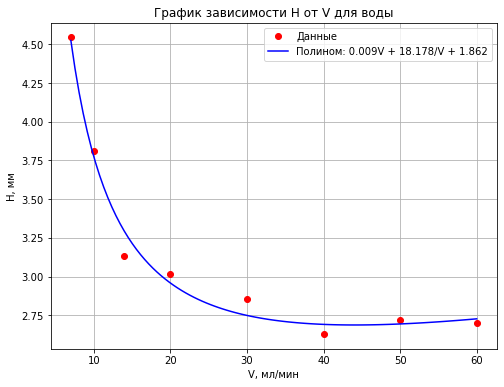
\includegraphics[width=0.75\linewidth]{Images/vd1.png}
    \caption{Зависимость $H(V)$ для воды }
    \label{fig:vd1}
\end{figure}
\begin{figure}[h]
    \centering
    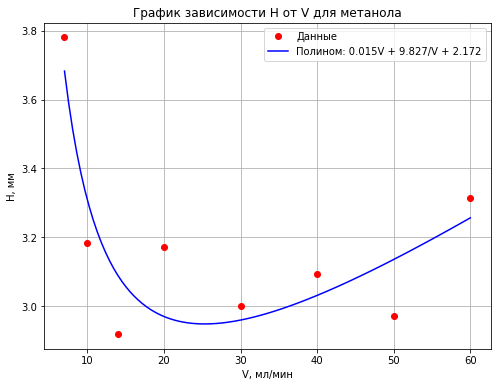
\includegraphics[width=0.75\linewidth]{Images/vd2.png}
    \caption{Зависимость $H(V)$ для метанола }
    \label{fig:vd2}
\end{figure}
\begin{figure}[h]
    \centering
    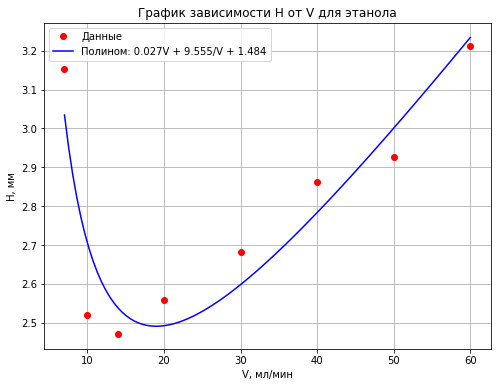
\includegraphics[width=0.75\linewidth]{Images/vd3.png}
    \caption{Зависимость $H(V)$ для этанола}
    \label{fig:vd3}
\end{figure}

\newpage
\par Оценим оптимальное значение для скорости потока (Таблица \ref{tab:v_opt}) исходя из минимума функции:

\begin{equation*}
    \frac{dH}{dv} = A - \frac{B}{v^2} = 0 \Rightarrow {v_{opt} = \sqrt{\frac{B}{A}}}
\end{equation*}
\begin{table}[h!]
\centering
\begin{tabular}{|l|l|l|l|}
\hline
             & Вода   & Метанол & Этанол \\ \hline
$v_{opt}$, мл/мин & 44,052 & 25,298  & 18,982 \\ \hline
\end{tabular}
\caption{Оптимальная скорость потока газа-носителя, мл/мин}
\label{tab:v_opt}
\end{table}
\newpage

\subsection{Оценка эффективного радиуса колонки}\;
По свободному члену в полиномиальной аппроксимации оценим эффективный радиус колонки (Таблица \ref{Радиус}):

\begin{table}[h!]
\centering
\caption{Эффективный радиус колонки}
\begin{tabular}{|l|l|l|l|}
\hline
Вещество & $H_2O$ & $CH_3OH$ & $C_2H_5OH$ \\ \hline
$\rho,\; $мм & 1,32 & 1,54 & 1,05 \\ \hline
\end{tabular}
\label{Радиус}
\end{table}

Отметим, что реальный (заявленный в методичке) радиус трубки установки равен $1,5$ мм.
\newpage
\section{Выводы}
\begin{itemize}
    \item В первой части работы по полученным данным мы рассчитали теплоты адсорбции на порапаке анализируемых веществ:
    \begin{table}[h!]
    \centering
    \begin{tabular}{|l|l|l|l|}
    \hline
    Вещество & $H_2O$ & $CH_3OH$ & $C_2H_5OH$ \\ \hline
    $Q,\;$ кДж/моль & $33,5 \pm 0,4$ & $38,4 \pm 0,5$ & $45,2 \pm 0,5$ \\ \hline
    \end{tabular}
    \end{table}
    \item Также мы сделали вывод о влиянии гидрофобной $-CH_2$ группы на величину теплоты адсорбции и отметили корреляцию между двумя этими параметрами: величина теплоты адсорбции растёт при увеличении гидрофобной части молекулы.
    \item Кроме того, мы качественно провели анализ полученных хроматограмм и предположили внешний вид изотерм адсорбции изучаемых веществ.
    \item Для каждого из веществ (вода, метанол, этанол) была определена разрешающая способность, число теоретических тарелок и ВЭТТ для разных скоростей потока газа-носителя.
    \item Построена зависимость ВЭТТ от скорости потока и проверено выполнение уравнения Ван-Деемтра. По минимуму функции найдены оптимумы скорости потока для какждого из тhёх веществ:
    \begin{table}[h!]
    \centering
    \begin{tabular}{|l|l|l|l|}
    \hline
             & Вода   & Метанол & Этанол \\ \hline
    $v_{opt}$, мл/мин & 44,052 & 25,298  & 18,982 \\ \hline
    \end{tabular}
    \end{table}
    \item По свободному члену в аппроксимациях оценили эффективный радиус колонки. Среднее от полученных значений равно $1,30$ мм. 
\end{itemize}
\end{document}
